%Antonio Giacomo Stradivari
%  A. Stradivarius écrit " Qui penserait que pour construire un violon, il faut d'abord tracer deux pentagones dans un cercle ? Mais les lois de l'harmonie découvertes par Platon, président aussi bien à la construction des figures géométriques qu'à la conception musicale, à cette conception abstraite de la musique-pensée ainsi qu'à l'établissement des proportions des instruments conçus pour la jouer".
\begin{figure}
\begin{center}
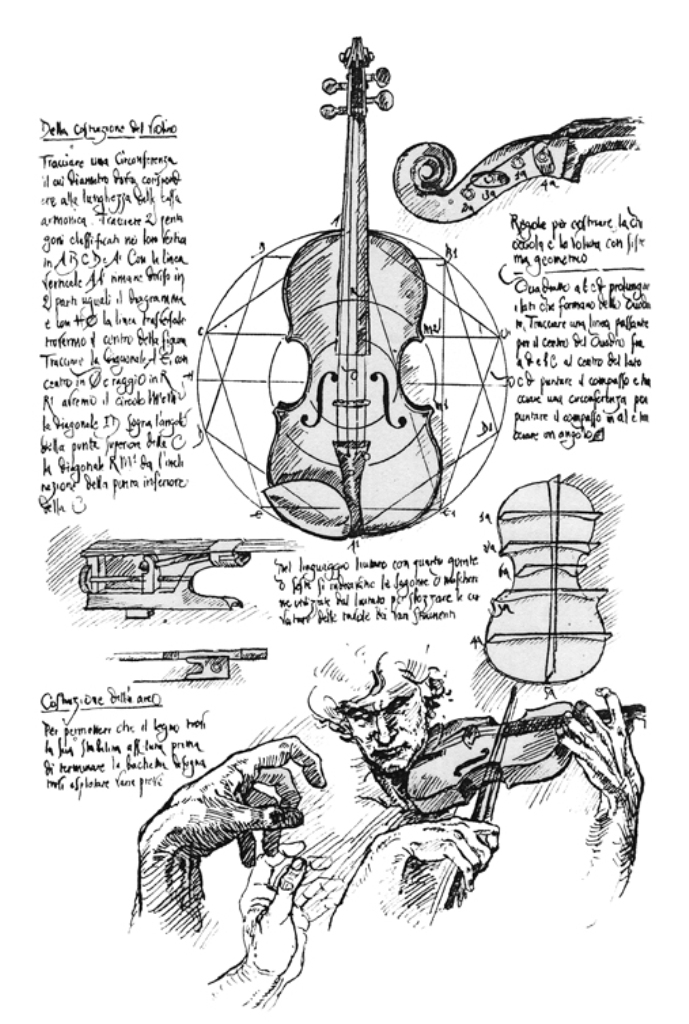
\includegraphics[width=12cm]{images/violon_carnet.jpg}
\end{center}
\end{figure}
